\documentclass[11pt]{article}
\usepackage[paperwidth=8.5in, paperheight=5.5in]{geometry}

\usepackage{../tjimo}

\begin{comment}
\def\answer{\comment}
\def\solution{\comment}
\def\solutionone{\comment}
\def\solutiontwo{\comment}
\end{comment}

\newcommand{\sevenpoints}{Time limit: 30 minutes.}
\newcommand{\righthead}{\fdbox{Round}{Guts}}

%%%%%%%%PUT THIS IN PREAMBLE%%%%%%%%%%
\usepackage{commath}
%\newcommand\floor[1]{\lfloor#1\rfloor}
%\newcommand\ceil[1]{\lceil#1\rceil}
\DeclareRobustCommand{\frac}[3][0pt]{%
  {\begingroup\hspace{#1}#2\hspace{#1}\endgroup\over\hspace{#1}#3\hspace{#1}}}

\begin{document}

%%%%%%%%%%%%%%%%%%%%%%%%%%%%%%%%%%%%%


\section*{Set 1}

\begin{problem}
What is 50\% of 10\% of 1000?
\end{problem}
\begin{answer}
\boxed{50}.
\end{answer}
\begin{solution}
10\% of 1000 is
$$\frac{10}{100} \times 1000 = 100.$$
50\% of 100 is
$$\frac{50}{100} \times 100 = \boxed{50}.$$
\end{solution}

\begin{problem}
I had 50 cookies yesterday but now I only have 30. If only two people—my brother, Frank, and my sister, Gabriella—ate my cookies, and I know Frank ate 8 of them, how many did my sister eat?
\end{problem}
\begin{answer}
\boxed{12} cookies.
\end{answer}
\begin{solution}
Since I had 50 cookies yesterday and now I only have 30, my siblings ate
$$50-30 = 20 \text{ cookies}.$$
Frank ate 8 of the 20 cookies, so Gabriella ate
$$20-8=\boxed{12} \text{ cookies}.$$
\end{solution}

\begin{problem}
If the area of a square is 64, what is its perimeter?
\end{problem}
\begin{answer}
\boxed{32}.
\end{answer}
\begin{solution}
The area of a square is its side length squared. We can check that its side length must be 8 since
$$8^2 = 64.$$
A square has 4 sides, so its perimeter is
$$4 \times \text{(side length)} = 4 \times 8 = \boxed{32}.$$
\end{solution}


\begin{problem}
Simplify $\frac{\sqrt{15^2+8^2}}{\sqrt{13^2-5^2}}$
\end{problem}
\begin{answer}
 \boxed{\frac{17}{12}}.
\end{answer}
\begin{solution}
We just compute the values:
\begin{align*}
\frac{\sqrt{15^2+8^2}}{\sqrt{13^2-5^2}} &= \frac{\sqrt{289}}{\sqrt{144}} \\
                    	&= \boxed{\frac{17}{12}}.
\end{align*}
\end{solution}

\eject

\section*{Set 2}

\begin{problem}How many primes are there that are less than 60?
\end{problem}

\begin{answer} \boxed{17}. \end{answer}
\begin{solution}
We list primes: Anything less than 60 and not divisible by 2, 3, 5 or 7 (unless the number itself is 2, 3, 5, or 7) is a prime less than 60. Listing these out, we have 2, 3, 5, 7, 11, 13, 17, 19, 23, 29, 31, 37, 41, 43, 47, 53, 59, for \boxed{17} primes less than 60.
\end{solution}

\begin{problem}Find the area of a circle with radius 6. Express your answer in terms of $\pi$.
\end{problem}

\begin{answer} $\boxed{36\pi}$. \end{answer}
\begin{solution}
Using the formula for the area of a circle of radius $r$, $A = \pi r^2$, the area is $\boxed{36 \pi}$.
\end{solution}

\begin{problem} Let $x \star y = x^2 - y^2$, and $x \uplus y = \sqrt{x^2 + y^2}$. Find $8 \star (5 \uplus 12)$.
\end{problem}

\begin{answer} $\boxed{-105}$. \end{answer}
\begin{solution}
Using the definitions provided, $8 \star (5 \uplus 12) = 8 \star \sqrt{12^2 + 5^2} = 8 \star 13 = 8^2 - 13^2 = 64 - 169 = \boxed{-105}.$
\end{solution}

\begin{problem}In how many different orders can I write the 4 letters in``WORD''?
\end{problem}

\begin{answer} \boxed{24}. \end{answer}
\begin{solution}
We can choose either ``W,'' ``O,'' ``R,'' or ``D'' for the first letter, for four choices. However, we only have three letters remaining for the second letter, two for the third letter, and the last remaining letter must go last. So, there are $4 \cdot 3 \cdot 2 \cdot 1 = 4! = \boxed{24}$ to arrange these letters.
\end{solution}

\eject

\section*{Set 3}

\begin{problem}
Compute $733^2-267^2$
\end{problem}
\begin{answer}
\boxed{466000}.
\end{answer}
\begin{solution}
We use the property $a^2-b^2 = (a+b)(a-b)$ so
$$(733+267)(733-267) = (1000)(466) = \boxed{466000}.$$
\end{solution}

\begin{problem}In a bizarre world far, far away, an apple is worth three bananas, an orange is worth 8 coconuts, and a coconut is worth 7 bananas. If an apple costs $\$1.50$, how many dollars does an orange cost?
\end{problem}
\begin{answer}
\boxed{28} dollars.
\end{answer}
\begin{solution}
We write the equations that describe the case of the problem, using $a, b, c, o$ to represent the price of apples, bananas, coconuts, and oranges respectively:
 \[
	\left\{
            	\begin{array}{ll}
              	a=3b\\
              	o=8c\\
              	c=7b \\
a=1.50
            	\end{array}
	\right\}
  \]
We can plug in the value of $a$ to find the price of bananas
$$b=\frac{a}{3} = \frac{1.50}{3} = 0.50$$
Then plug in $b$ to find $c,$
$$c=7b = 7(0.50) = 3.50.$$
And finally plug in $c$ to find $o$,
$$o=8c=8(3.50)=28.$$
So our final answer is $\boxed{\$ 28}$.
\end{solution}


\begin{problem}What is the value of $\sqrt{x^{3}+3y}$ if $x=7$ and $y=6$?
\end{problem}
\begin{answer}
\boxed{19}.
\end{answer}
\begin{solution}
We substitute $x=7, y=6$ into the expression,
$$\sqrt{x^{3}+3y}=\sqrt{7^3+3(6)}=\sqrt{343+18}=\sqrt{361}=\boxed{19}.$$
\end{solution}

\begin{problem}Find the smallest four digit number that is divisible by 2, 3, and 11.
\end{problem}
\begin{answer}
\boxed{1056}.
\end{answer}
\begin{solution}
We first find the smallest number that is divisible by 2, 3, and 11. That number is simply the least common multiple of the three numbers, which is
$$2\cdot 3\cdot 11=66$$
Since any multiple of 66 will be divisible by 2, 3, and 11, we need to find the smallest multiple of 66 that is a four digit number. This can be found by
$$\floor{\frac{1000}{66}}=15$$
So $66 \cdot 15$ will be less than 100 and the next multiple will be the first multiple greater than 1000 (and thus a four digit number). $66 \cdot 16 = \boxed{1056}.$
\end{solution}

\eject

\section*{Set 4}

\begin{problem}
How many non-congruent isosceles triangles with positive area and integer side lengths have perimeter 14?
\end{problem}
\begin{answer}
\boxed{3}.
\end{answer}
\begin{solution}
Note that if the sides of the triangle are $a$, $a$, and $b$, we have $b = 14 - 2a = 2(7 - a)$. Since $0 < b < 14$, $0 < a < 7$. However, the triangle inequality also requires that $a + a > b = 14 - 2a$, so $4a > 14$ and $a \geq 4$ because $a$ is an integer. This leaves the cases $a = 4, 5, 6$, all of which are possible: Triangles with side lengths 4-4-6, 5-5-4, and 6-6-2 are all valid. So, there are \boxed{3} such isosceles triangles.
\end{solution}

\begin{problem}
What are the sum of the prime factors of $3^{8}-1$?
\end{problem}
\begin{answer}
\boxed{48}.
\end{answer}
\begin{solution}
We can use the property $a^2-b^2 = (a+b)(a-b)$ to make our lives easier (instead of calculating $3^8-1$ all the way out and looking for factors).
$$3^8-1 = (3^4+1)(3^4-1) = (82)(3^2+1)(3^2-1)=(2)(41)(10)(8)=2^5 \cdot 5 \cdot 41$$
Our prime factors are 2, 5, and 41, so our answer is
$$2+5+41 = \boxed{48}.$$
\end{solution}

\begin{problem}
How many integer solutions of $x$ exist for $\left| 2x-21 \right| \leq 7$?
\end{problem}
\begin{answer}
\boxed{8}.
\end{answer}
\begin{solution}
We have two cases. When $2x-21$ is positive and when it is negative. \\
\textbf{Case 1:} $2x-21$ is positive.
So we can write
\begin{align*}
2x-21 &\leq 7 \\
2x &\leq 28 \\
x &\leq 14.
\end{align*}
\textbf{Case 2:} $2x-21$ is negative.
So we can write
\begin{align*}
2x-21 &\geq -7 \\
2x &\geq 14 \\
x &\geq 7.
\end{align*}
So we have
$$7 \leq x \leq 14.$$
and we have $x = 7, 8, \cdots, 13, 14$ and $\boxed{8}$ solutions for $x$.
\end{solution}

\begin{problem}
A stock began at \$1000. If throughout the year it increased in value by 10\%, then increased by 30\%,
and finally decreased by 40\%, what was its final value in dollars?
\end{problem}
\begin{answer}
\boxed{\$858}. 
\end{answer}
\begin{solution}
The following gives the value of the stock over the year:
$$ \$1000 \times \frac{11}{10} \times \frac{13}{10} \times \frac{6}{10} = 11 \times 13 \times 6 = \boxed{\$858}.$$
\end{solution}

\eject

\section*{Set 5}

\begin{problem}Three VMT officers can write a lecture in two seconds. How many seconds would it take 5 VMT officers to write 10 lectures?
\end{problem}

\begin{answer} \boxed{12} seconds. \end{answer}
\begin{solution}
Since 3 VMT officers can write a lecture in two seconds, 3 VMT officers write half of a lecture in one second, so 1 VMT officer writes $\displaystyle \frac{1}{6}$ of a lecture in one second. So, 5 VMT officers write $\displaystyle \frac{5}{6}$ of a lecture in one second and 5 VMT officers can write 10 lectures in $\displaystyle \frac[5pt]{10}{\frac{5}{6}} = \boxed{12}$ seconds.
\end{solution}

\begin{problem}Fill in the blank in the following sequence: $1, \frac{3}{2}, \frac{7}{4}, \frac{15}{8}, \frac{31}{16}, \underline{\phantom{aaaa}}.$
\end{problem}

\begin{answer} $\boxed{\displaystyle \frac{63}{32}}$. \end{answer}
\begin{solution}
Notice that the $n^{\text{th}}$ term of the sequence is given by $\displaystyle 2 - \frac{1}{2^{n-1}}$. The next term is the $6^{\text{th}}$ term, so it is $\displaystyle 2 - \frac{1}{2^{5}} = 2 - \frac{1}{32} = \frac{64 - 1}{32} = \boxed{\frac{63}{32}}$.
\end{solution}

\begin{problem} Samel is a crazy kid who is only happy if he has his favorite number of camels. Four of these are purple, and the others are white. Samel knows that when he has his favorite number of camels, three times the number of white camels equals the sum of the number of white camels and the total number of camels. What is Samel's favorite number of camels?
\end{problem}

\begin{answer} \boxed{8} camels. \end{answer}
\begin{solution}
Let $x$ be the number of camels. Then, there are 4 purple camels and $x - 4$ white camels. Writing the condition given, $3(x - 4) = x - 4 + x$. Solving, $x = 3 \cdot 4 - 4 = \boxed{8}$ camels.
\end{solution}

\begin{problem} Compute the number of factors of 900.
\end{problem}

\begin{answer} \boxed{27}. \end{answer}
\begin{solution}
Note that $900 = 2^2 \cdot 3^2 \cdot 5^2$, so it has $(2 + 1)(2 + 1)(2 + 1) = \boxed{27}$ factors.
\end{solution}

\eject

\section*{Set 6}

\begin{problem}What is the smallest positive integer that has a remainder of 2 when divided by 7 and 1 when divided by 9?
\end{problem}
\begin{answer}
\boxed{37}.
\end{answer}
\begin{solution}
We can list out all numbers which satisfy remainder 2 when divided by 7, and remainder 1 when divided by 9, and find the smallest number that appears on both lists.
\begin{align*}
2, 9, 16, 23, 30, \underline{37} \\
1, 10, 19, 28, \underline{37}
\end{align*}
So our answer is $\boxed{37}$.
\end{solution}

\begin{problem}On a $5 \times 7$ grid, Charles can only move upwards or to the right and can only move along gridlines. In how many ways can he move from the lower left corner to the top right corner?
\end{problem}
\begin{answer}
\boxed{792} ways.
\end{answer}
\begin{solution}
We know in order to get from corner to corner, Charles will have to move right 5 times, and move up 7 times. Therefore, we can think of his sequence of steps from going from corner to corner as a sequence of 5 R's and 7 U's. This is just
$$\frac{(5+7)!}{5!7!}=\frac{12!}{5!7!} = \frac{12 \cdot 11 \cdot 10 \cdot 9 \cdot 8}{5 \cdot 4 \cdot 3 \cdot 2 \cdot 1} = \boxed{792}.$$
\end{solution}

\begin{problem}What are the last two digits of $7^{2015}$?
\end{problem}
\begin{answer}
\boxed{43}.
\end{answer}
\begin{solution}
We begin by listing the last two digits of some smaller powers of 7.
\begin{align*}
7^1 &= 07 \\
7^2 &= 49 \\
7^3 &= 43 \\
7^4 &= 01 \\
7^5 &= 07
\end{align*}
We see that the last two digits of seven repeat every four powers. 2015 has a remainder of 3 when divided by 4, so our answer is $\boxed{43}$.
\end{solution}

\begin{problem}If $3^{2x-4} = 4$, what is the value of $3^{x}$?
\end{problem}
\begin{answer}
\boxed{18}.
\end{answer}
\begin{solution}
Since solving for $x$ in the first equation is not very nice, we instead look for ways to manipulate the first equation.
\begin{align*}
3^{2x-4} &= 3^{2x} \cdot 3^{-4} \\
&= (3^x)^2 \cdot 3^{-4}.
\end{align*}
We now see we can isolate  $3^{x}$ and thus solve for it.
\begin{align*}
(3^x)^2 \cdot 3^{-4} &= 4 \\
(3^x)^2 &= 324 \\
3^x &= \boxed{18}.
\end{align*}
\end{solution}

\eject

\pdfpageheight=11in

\section*{Set 7}

\begin{problem}  Bo Schmoe is raising farm animals, but only has mos and joes. A \emph{mo} has 2 heads and a \emph{joe} has 3 heads. If Bo has 29 animals and these animals have 71 heads total, what is the absolute value of the difference between the number of mos and the number of joes on Bo Schmoe's farm?
\end{problem}

\begin{answer} \boxed{3}. \end{answer}
\begin{solution}
Let Bo have $x$ mos and $y$ joes. Then, we can set up the system
\begin{align*}
x + y &= 29 \\
2x + 3y &= 71
\end{align*}
Subtracting twice the first equation from the second, we have $(2x + 3y) - 2(x + y) = 71 - 2 \cdot 29$, so $y = 13$. As $x + y = 29$, $x = 16$. Our answer is $\left| x - y \right| = 16 - 13 = \boxed{3}$.
\end{solution}

\begin{problem} Victoria and Katherine are sharing a circular pizza. However, they only have a very bad knife that can only making 3 straight cuts before breaking. If they cannot rearrange the pizza pieces until they have made all the cuts, what is the largest number of pieces Victoria and Katherine can cut the pizza into?
\end{problem}

\begin{answer} \boxed{7}. \end{answer}
\begin{solution}
Note that each cut at most doubles the number of pieces. Now, consider the following two cases:
\begin{enumerate}
\item The first two cuts do not intersect in the pizza. Then, these first two cuts must divide the pizza into 3 pieces. The third cut can double this, producing 6 pieces.
\item The first two cuts intersect in the pizza, so they cut the pizza into 4 pieces. Then, the third cut can pass through 3 of these pieces, adding 3 pieces, for a total of 7. Note that because the third cut cannot pass through all 4 pieces, we cannot have eight pieces.
\end{enumerate}
Taking the maximum of these two cases, Victoria and Katherine can cut the pizza into \boxed{7} pieces maximum.
\end{solution}

\begin{problem} What is the  $5^{\text{th}}$ smallest number with 5 factors?
%Katherine Cheng
\end{problem}

\begin{answer} \boxed{14641}. \end{answer}
\begin{solution}
The only numbers with 5 factors are the fourth powers of primes. The $5^{\text{th}}$ prime is 11. By the binomial theorem, $11^4 = 14641$, giving the answer of \boxed{14641}.
\end{solution}

\begin{problem} In how many ways can the letters in ``EFFERSON'' be arranged?
\end{problem}

\begin{answer} \boxed{10080}. \end{answer}
\begin{solution}
Note that we have 2 E's, 2 F's, and all other letters are distinct. So, the number of ways to arrange the letters is the number of ways to arrange 8 distinct letters, 8!, divided by the number of ways to switch the 2 E's times the number of ways to switch the 2 F's. This expession is $\displaystyle \frac{8 \cdot 7 \cdot 6 \cdot 5 \cdot 4 \cdot 3 \cdot 2 \cdot 1}{2 \cdot 2} = 8 \cdot 7 \cdot 6 \cdot 5 \cdot 3 \cdot 2 = \boxed{10080}$.
\end{solution}

\eject

\pdfpageheight=5.5in

\section*{Set 8}

\begin{problem}Jendy is shipping herself down a river. Paddling furiously in her cardboard box, she travels downstream to her chosen man in 3 hours. However, when she realizes that she chose the wrong man, it takes her 5 hours to paddle upstream to her starting point. What is the ratio of Jendy's paddling speed in still water to the speed of the current?
\end{problem}

\begin{answer} \boxed{4}. \end{answer}
\begin{solution}
Let Jendy have speed $j$, the current have speed $c$, and the distance she travels to be $d$. Then, $3(j + c) = d = 5(j- c),$ and $8c = 2j$, so the desired ratio $\displaystyle \frac{j}{c} = \frac{8}{2} = \boxed{4}.$
\end{solution}.

\begin{problem}
Everyone in VMT is either an Akshaj, who always tells the truth, or a Franklyn, who always lies. A group of confused freshmen meets VMT members Will, Michael, Ruiran, and Alex. The VMT members say the following:
	\begin{itemize}
    	\item Will says, ``Only Franklyns get sweaty.''
    	\item Michael says, ``Will is so rich that he's a Franklyn.''
    	\item Ruiran says, ``Will does not get sweaty.''
    	\item Alex says, ``Both Will and I are Franklyns.''
	\end{itemize}
	How many of the 4 VMT members are Franklyns?
\end{problem}

\begin{answer} \boxed{2}. \end{answer}
\begin{solution}
Notice that neither an Akshaj nor a Franklyn can say that they are a Franklyn. So, Alex is lying and is a Franklyn. That means that since it is not true that both Will and Alex are Franklyns and Alex is a Franklyn, Will must be an Akshaj. Therefore, Michael is a Franklyn. Since Will is an Akshaj and he says only Franklyns get sweaty, he does not get sweaty, and Ruiran is telling the truth. So, only Michael and Alex are Franklyns, and our answer is \boxed{2}.
\end{solution}

\begin{problem} How many convex hexagons are there drawn below? A polygon is said to be convex if all of its interior angles have measure less than $180^{\circ}$.

\begin{center}
\begin{asy}
size(6cm);

pair a1=(5,0), a2=(6,0), a3=(7,0), a4=(8, 0);
pair b1=(0, 8.66), b2=(0.5, 9.526), b3=(1, 10.39), b4=(1.5, 11.26);
draw(a1--b1, linewidth(1.5));
draw(a2--b2, linewidth(1.5));
draw(a3--b3, linewidth(1.5));
draw(a4--b4, linewidth(1.5));

pair c1=(5,17.32), c2=(6,17.32), c3=(7,17.32), c4=(8, 17.32);
pair d1=(0, 8.66), d2=(0.5, 7.794), d3=(1, 6.93), d4=(1.5, 6.06);
draw(c1--d1, linewidth(1.5));
draw(c2--d2, linewidth(1.5));
draw(c3--d3, linewidth(1.5));
draw(c4--d4, linewidth(1.5));

pair e1=(5,17.32), e2=(4.5,16.455), e3=(4,15.59), e4=(3.5, 14.72);
pair f1=(15,17.32), f2=(15.5,16.455), f3=(16,15.59), f4=(16.5, 14.72);
draw(e1--f1, linewidth(1.5));
draw(e2--f2, linewidth(1.5));
draw(e3--f3, linewidth(1.5));
draw(e4--f4, linewidth(1.5));

pair g1=(12,17.32), g2=(13,17.32), g3=(14,17.32), g4=(15, 17.32);
pair h1=(20, 8.66), h2=(19.5, 7.794), h3=(19, 6.93), h4=(18.5, 6.06);
draw(g4--h1, linewidth(1.5));
draw(g3--h2, linewidth(1.5));
draw(g2--h3, linewidth(1.5));
draw(g1--h4, linewidth(1.5));

pair i1=(15,0), i2=(14,0), i3=(13,0), i4=(12, 0);
pair j1=(20, 8.66), j2=(19.5, 9.526), j3=(19, 10.39), j4=(18.5, 11.26);
draw(i1--j1, linewidth(1.5));
draw(i2--j2, linewidth(1.5));
draw(i3--j3, linewidth(1.5));
draw(i4--j4, linewidth(1.5));

pair k1=(5,0), k2=(4.5,0.866), k3=(4,1.73), k4=(3.5, 2.60);
pair l1=(15,0), l2=(15.5,0.866), l3=(16,1.73), l4=(16.5, 2.60);
draw(k1--l1, linewidth(1.5));
draw(k2--l2, linewidth(1.5));
draw(k3--l3, linewidth(1.5));
draw(k4--l4, linewidth(1.5));
\end{asy}
\end{center}

\end{problem}

\begin{answer} \boxed{4096}. \end{answer}
\begin{solution}
Note that for each side of the hexagon, we may choose any of the 4 segments there grouped together to be that side. As there are 6 sides and we have 4 choices for each side, we have $4 \cdot 4 \cdot 4 \cdot 4 \cdot 4 \cdot 4 = 4^6 = \boxed{4096}$.
\end{solution}

\begin{problem}If $\frac{1}{x} + 3 = \sqrt{10}$, what is $x$ to the nearest integer?
\end{problem}

\begin{answer}
\boxed{6}.
\end{answer}
\begin{solution}
Since we want to know what $x$ is closest to, we can subtract both sides by 3 and take the reciprocal of both sides of the given equation.
$$x = \frac{1}{\sqrt{10}-3}$$.
We now rationalize the denominator
\begin{align*}
x &= \frac{1}{\sqrt{10}-3} \times \frac{\sqrt{10}+3}{\sqrt{10}+3} \\
&= \frac{\sqrt{10}+3}{10-9} \\
&= \sqrt{10}+3.
\end{align*}
We see that $\sqrt{10}$ rounds down to 3 because $3.5^2 = 12.25$ so our answer is $3+3=\boxed{6}$.
\end{solution}

\eject

\section*{Set 9}

\begin{problem}Find the area of the shaded region.
	\begin{center}
	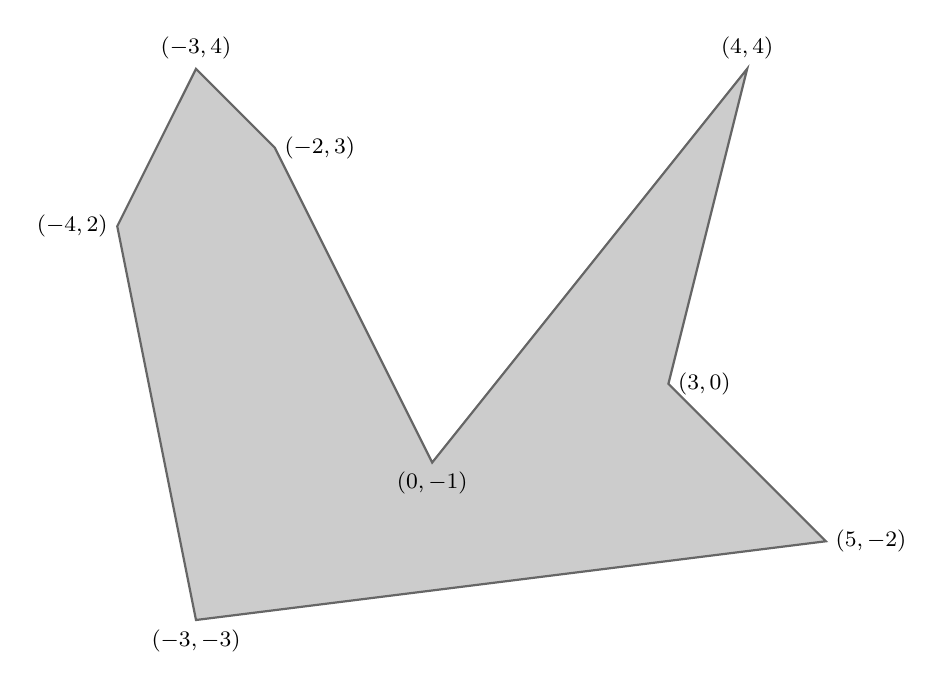
\begin{tikzpicture}
	\filldraw[color=black!60, fill=black!20, thick] (4, 4) -- (0, -1) -- (-2, 3) -- (-3, 4) -- (-4, 2) -- (-3, -3) -- (5, -2) -- (3, 0) -- cycle;
	\fill[black,font=\footnotesize](4, 4) node [above] {$(4, 4)$}
	(0, -1) node [below] {$(0, -1)$}
	(-2, 3) node [right] {$(-2, 3)$}
	(-3, 4) node [above] {$(-3, 4)$}
	(-4, 2) node [left] {$(-4, 2)$}
	(-3, -3) node [below] {$(-3, -3)$}
	(5, -2) node [right] {$(5, -2)$}
	(3, 0) node [right] {$(3, 0)$};
	\end{tikzpicture}
	\end{center}
\end{problem}

\begin{answer} $\boxed{31}$. \end{answer}
\begin{solution}
We consider the rectangle with vertices $(-4, -3), (-4, 4), (5, 4),$ and $(5, -3)$. The area of the shaded area is the area of this rectangle minus the areas that are not shaded. These areas are as follows:
\begin{itemize}
	\item The triangle with vertices $(-4, -3), (-4, 2),$ and $(-3, 3)$ has area $\frac{1}{2} 1 \cdot 5 = \frac{5}{2}$.
	\item The triangle with vertices $(-4, 2), (-4, 4),$ and $(-3, 4)$ has area $\frac{1}{2} 1 \cdot 2 = 1$.
	\item The triangle with vertices $(-3, 4), (-2, 4),$ and $(-2, 3)$ has area $\frac{1}{2} 1 \cdot 1 = \frac{1}{2}$.
	\item The trapezoid with vertices $(-2, 4), (0, 4), (0, -1),$ and $(-2, 3)$ has area $\frac{1}{2} 2(1 + 5) = 6$.
	\item The triangle with vertices $(0, 4), (4, 4),$ and $(0, -1)$ has area $\frac{1}{2} 4 \cdot 5 = 10$.
	\item The trapezoid with vertices $(4, 4), (5, 4), (5, 0),$ and $(3, 0)$ has area $\frac{1}{2} 	4(1+2) = 6$.
	\item The triangle with vertices $(3, 0), (5, 0),$ and $(5, -2)$ has area $\frac{1}{2} 2 \cdot 2 = 2$,
	\item The triangle with vertices $(5, -2), (5, -3),$ and $(-3, -3)$ has area $\frac{1}{2} 8 \cdot 1 = 4$.
\end{itemize}
Subtracting the sum of these areas from that of the rectangle, the area of the shaded region is $\displaystyle 9 \cdot 7 - (\frac{5}{2} + 1 + \frac{1}{2} + 6 + 10 + 6 + 2 + 4) = 63 - 32 =\boxed{31}$.
\end{solution}

\begin{problem}The time is now 4:00 on an analog clock (a normal clock with hands). In how many minutes will the minute and hour hands of this clock be exactly together? Give your answer to the nearest minute. %variation would be the time is now 4:00 and the minute hand is 120 degrees behind the hour hand. At what time will the minute hand be 120 degrees ahead of the hour hand?
\end{problem}

\begin{answer}
$\boxed{22}$ minutes.
\end{answer}
\begin{solution}
At 4:00, the hour hand is $12^{\circ}$ ahead of the minute hand. Since the rate of the minute hand is $360^{\circ} / 60 \text{min} = 6 ^{\circ} / \text{min}$ and the rate of the hour hand is $30 ^{\circ} / 60 \text{min}= \frac{1}{2} ^{\circ} / \text{min}$, the minute hand ``catches up'' at a rate of
$$6 ^{\circ} / \text{min}-\frac{1}{2} ^{\circ} \text{min} = \frac{11}{2} ^{\circ} / \text{min}$$
So the time it takes the minute hand to close the $120 ^{\circ}$ gap is
$$\frac{120 ^{\circ}}{\frac{11}{2} ^{\circ} / \text{min}} = \frac{240}{11} \text{min} = 21 \frac{9}{11} \text{min}.$$
Rounding to the nearest minute, our answer is $\boxed{22}$ minutes.
\end{solution}

\begin{problem}Evaluate $1\cdot2^{0} + 2\cdot2^1 + 3\cdot2^2 +\cdots+12\cdot2^{11}$
\end{problem}

\begin{answer}
\boxed{45057}.
\end{answer}
\begin{solution}
We set the sum equal to $S$. If we multiply $S$ by 2,
\begin{align*}
S = 1\cdot2^{0} + 2\cdot2^1 + 3\cdot2^2 +\cdots+12\cdot2^{11} \\
2S = 1\cdot2^{1} + 2\cdot2^2 + 3\cdot2^3 +\cdots+12\cdot2^{12}
\end{align*}
If we subtract the original equation from the second one, we see that we can get some terms and a geometric sequence, which we can easily calculate:
\begin{align*}
2S-S=S &= -(2^0 + 2^1+2^2+\cdots+2^{11})+12 \cdot 2^{12} \\
&= 12\cdot 2^{12}- (\frac{2^{12}-1}{2-1}) \\
&= 12\cdot 2^{12}-2^{12}+1 \\
&= 11 \cdot 2^{12} + 1 \\
&= 11(4096) + 1 = 45056+1 = \boxed{45057}.
\end{align*}
\end{solution}

\begin{problem}What is the remainder when $3^{178}$ is divided by 30?
\end{problem}
\begin{answer}
\boxed{9}.
\end{answer}
\begin{solutionone}
We can find integers $a$ and $b$, $0 \leq b \leq 9$, such that
$$3^{177} = 10a+b$$
and therefore
$$3^{177} \cdot 3 = 3(10a+b) = 30a+3b$$
So our remainder is $3b$. Since
$$3^2 = 9 \equiv -1 \pmod{10},$$
we have:
\begin{align*}
3^{177} &\equiv (9)^{88} \cdot 3  \pmod{10} \\
&\equiv (-1)^{88} \cdot 3 \pmod{10} \\
&\equiv 3 \pmod{10}.
\end{align*}
So we see $b=3$ and our remainder when we divide $3^{178}$ by 30 is $3b = \boxed{9}$.
\end{solutionone}
\begin{solutiontwo}
Since 3 is not relatively prime to 30, we cannot use Euler's totient theorem so we proceed by computation. \par
We note that
$$3^3 = 27 \equiv -3 \pmod{30}.$$
So
\begin{align*}
3^{178} &\equiv (27)^{59} \cdot 3 \pmod{30} \\
&\equiv (-3)^{59} \cdot 3 \pmod{30}\\
&\equiv -(3)^{59} \cdot 3 \pmod{30}\\
&\equiv -(27)^{19} \cdot 3^2 \cdot 3 \pmod{30}\\
&\equiv 3^{19} \cdot (-3) \pmod{30}\\
&\equiv (27)^6 \cdot 3 \cdot -3  \pmod{30}\\
&\equiv (-3)^6 \cdot -9 \pmod{30}\\
&\equiv (27)^2 \cdot -9 \pmod{30}\\
&\equiv -81 \pmod{30}\\
&\equiv \boxed{9} \pmod{30}.
\end{align*}
\end{solutiontwo}

\end{document}